% VUT FIT MITAI
% MSZ 2021/2022
% Author: Vladimir Dusek
% Login: xdusek27

%%%%%%%%%%%%%%%%%%%%%%%%%%%%%%%%%%%%%%%%%%%%%%%%%%%%%%%%%%%%%%%%%%%%%%%%%%%%%%%%

% Path to figures
\graphicspath{{prl/distribuovany_broadcast/figures}}

%%%%%%%%%%%%%%%%%%%%%%%%%%%%%%%%%%%%%%%%%%%%%%%%%%%%%%%%%%%%%%%%%%%%%%%%%%%%%%%%

\chapter{PRL~--~Distribuovaný broadcast, synchronizace v distribuovaných systémech.}

%%%%%%%%%%%%%%%%%%%%%%%%%%%%%%%%%%%%%%%%%%%%%%%%%%%%%%%%%%%%%%%%%%%%%%%%%%%%%%%%

\section{Zdroje}

\begin{compactitem}
    \item \path{PRL_12_bcast_slidy.pdf}
    \item \textit{Otázka souvisí s prvními 2 otázkami z PDI.}
\end{compactitem}

%%%%%%%%%%%%%%%%%%%%%%%%%%%%%%%%%%%%%%%%%%%%%%%%%%%%%%%%%%%%%%%%%%%%%%%%%%%%%%%%

\section{Úvod a kontext}

\begin{compactitem}
    \item \textit{Stejný úvodní text jako pro otázku~\ref{chapter_pdi_koordinator}.}

    \item Mějme množinu procesů v~rámci distribuovaného systému. Řešíme problém  nalezení shody na nějaké věci (synchronizační problém). Problém můžeme rozdělit na dvě situace: \begin{compactitem}
        \item \textbf{Problém volby koordinátora} -- Výběr jednoho z~procesů, který bude vedoucím procesem (koordinátor). Tento proces pak může vykonat určitou činnost nebo může sloužit ostatním procesům k~realizaci  význačné role v~systému.

        \item \textbf{Problém vzájemného vyloučení} -- Předpokládejme, že konkrétní zdroj může v~daném okamžiku používat pouze jeden proces. Tento problém se běžně vyskytuje ve víceprocesorových systémech, ale také v~distribuovaných systémech.
    \end{compactitem}

    \item Synchronizační problémy lze v~rámci operačních systémů nebo multiprocesorových systémů řešit pomocí provádění atomických operací, sdílené paměti apod. -- je pro ně podpora v~rámci operačního systému nebo hardwaru. V~distribuovaných systémech takovéto prostředky nejsou často k dispozici, proto se synchronizační problémy řeší pomocí zasílání zprav, resp. algoritmicky.
\end{compactitem}

%%%%%%%%%%%%%%%%%%%%%%%%%%%%%%%%%%%%%%%%%%%%%%%%%%%%%%%%%%%%%%%%%%%%%%%%%%%%%%%%

\section{Synchronizace}

\begin{compactitem}
    \item Synchronizace zaručuje (částečné) uspořádání mezi událostmi -- zajištění uspořádání některých událostí v systému v nějakém pořadí.

    \item V distribuovaných systémech se sdílenou pamětí můžeme použít semafory nebo monitory.

    \item V distribuovaných systémech se sdíleným prostředkem, jako je například nástěnka, můžeme synchronizaci realizovat například pomocí systému ADA nebo LINDA.

    \item Ale pokud chceme zajistit synchronizaci pouze pomocí předáváním zpráv potřebujeme algoritmy.

    \item Požadavky: \begin{compactitem}
        \item \textbf{Kauzalita} -- uspořádání v reálném čase $\sim$ uspořádání dle logických hodin nebo časových razítek (\uv{korektní chování z pohledu uživatele}).
        \item Všechny procesy uspořádávají události v tom samém pořadí.
    \end{compactitem}
\end{compactitem}

%%%%%%%%%%%%%%%%%%%%%%%%%%%%%%%%%%%%%%%%%%%%%%%%%%%%%%%%%%%%%%%%%%%%%%%%%%%%%%%%

\section{Synchronizace globálním (reálným, fyzickým) časem}

\begin{compactitem}
    \item Využívá se fyzický globální čas.
    \item Předpokládá se, že komunikace dotaz-odpověď (návratový čas) je dostatečně krátká.
    \item Hlavní uzel si vyžádá od všech hodnotu posunu vůči svému aktuálnímu času.
    \item Následně vypočte průměrnou hodnotu posunu a z té posuny pro jednotlivé uzly.

    \item Seznam algoritmů: \begin{compactitem}
        \item Berkley algoritmus
        \item Marzullo-ův algoritmus
    \end{compactitem}
\end{compactitem}

\subsection{Network Time Protocol (NTP)}

\begin{compactitem}
    \item Synchronizace v síti na různých úrovních (stratech).
    \item Komunikace přes UDP.
    \item Universal Coordinated Time (UCT) -- Spolehlivý a přesný zdroj času, založen na atomových hodinách (nezávislý rotaci Země teoreticky).

    \item Řešíme: \begin{compactitem}
        \item Zpoždění (\textit{delay}, RTT, \textit{round trip time}) mezi dvěma uzly.
        \item Posunutí (\textit{offset}) dvou uzlů vzájemně od sebe.
    \end{compactitem}

    \begin{figure}[H]
        \centering
        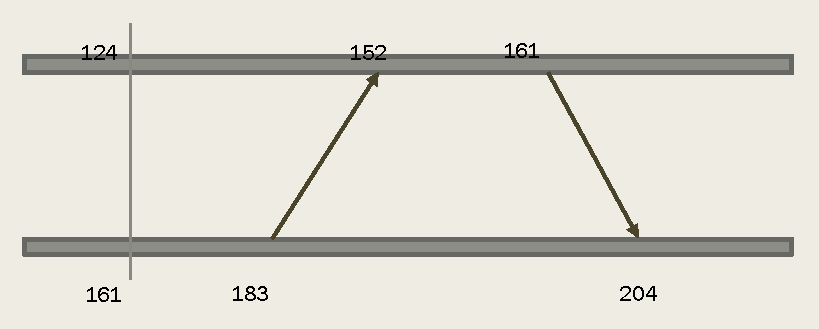
\includegraphics[width=1\linewidth]{ntp_priklad.pdf}
        \caption{Příklad uzlů s fyzickým časem. Zpoždění: $RTT = 152-183 + 204-161= -31 +43 = 12 $, posunutí: $o = \frac{1}{2} (152-183+161-204) = -37 $.}
    \end{figure}

    \begin{figure}[H]
        \centering
        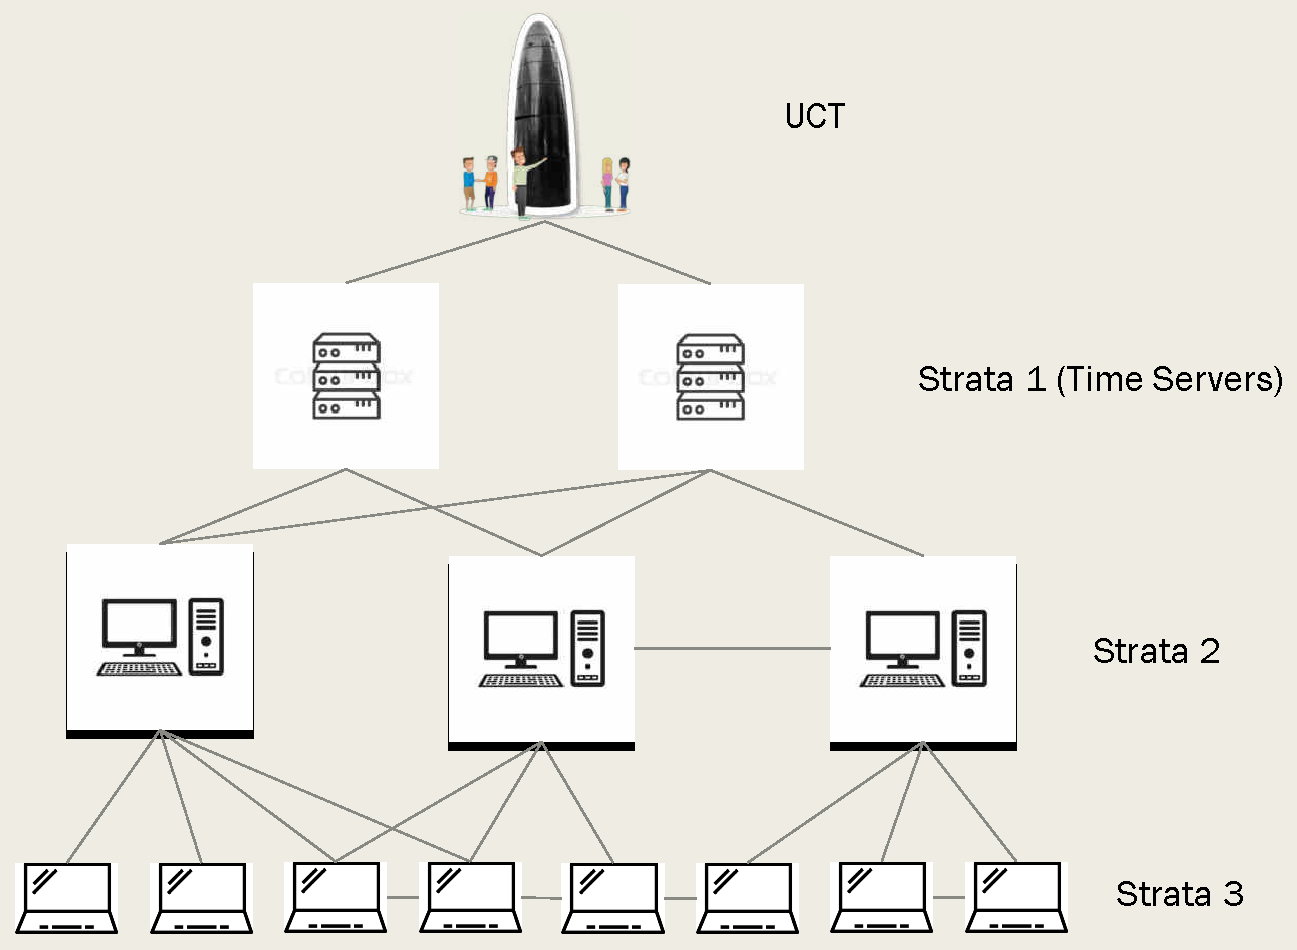
\includegraphics[width=1\linewidth]{ntp.pdf}
        \caption{Úrovně NTP.}
    \end{figure}

    \begin{figure}[H]
        \centering
        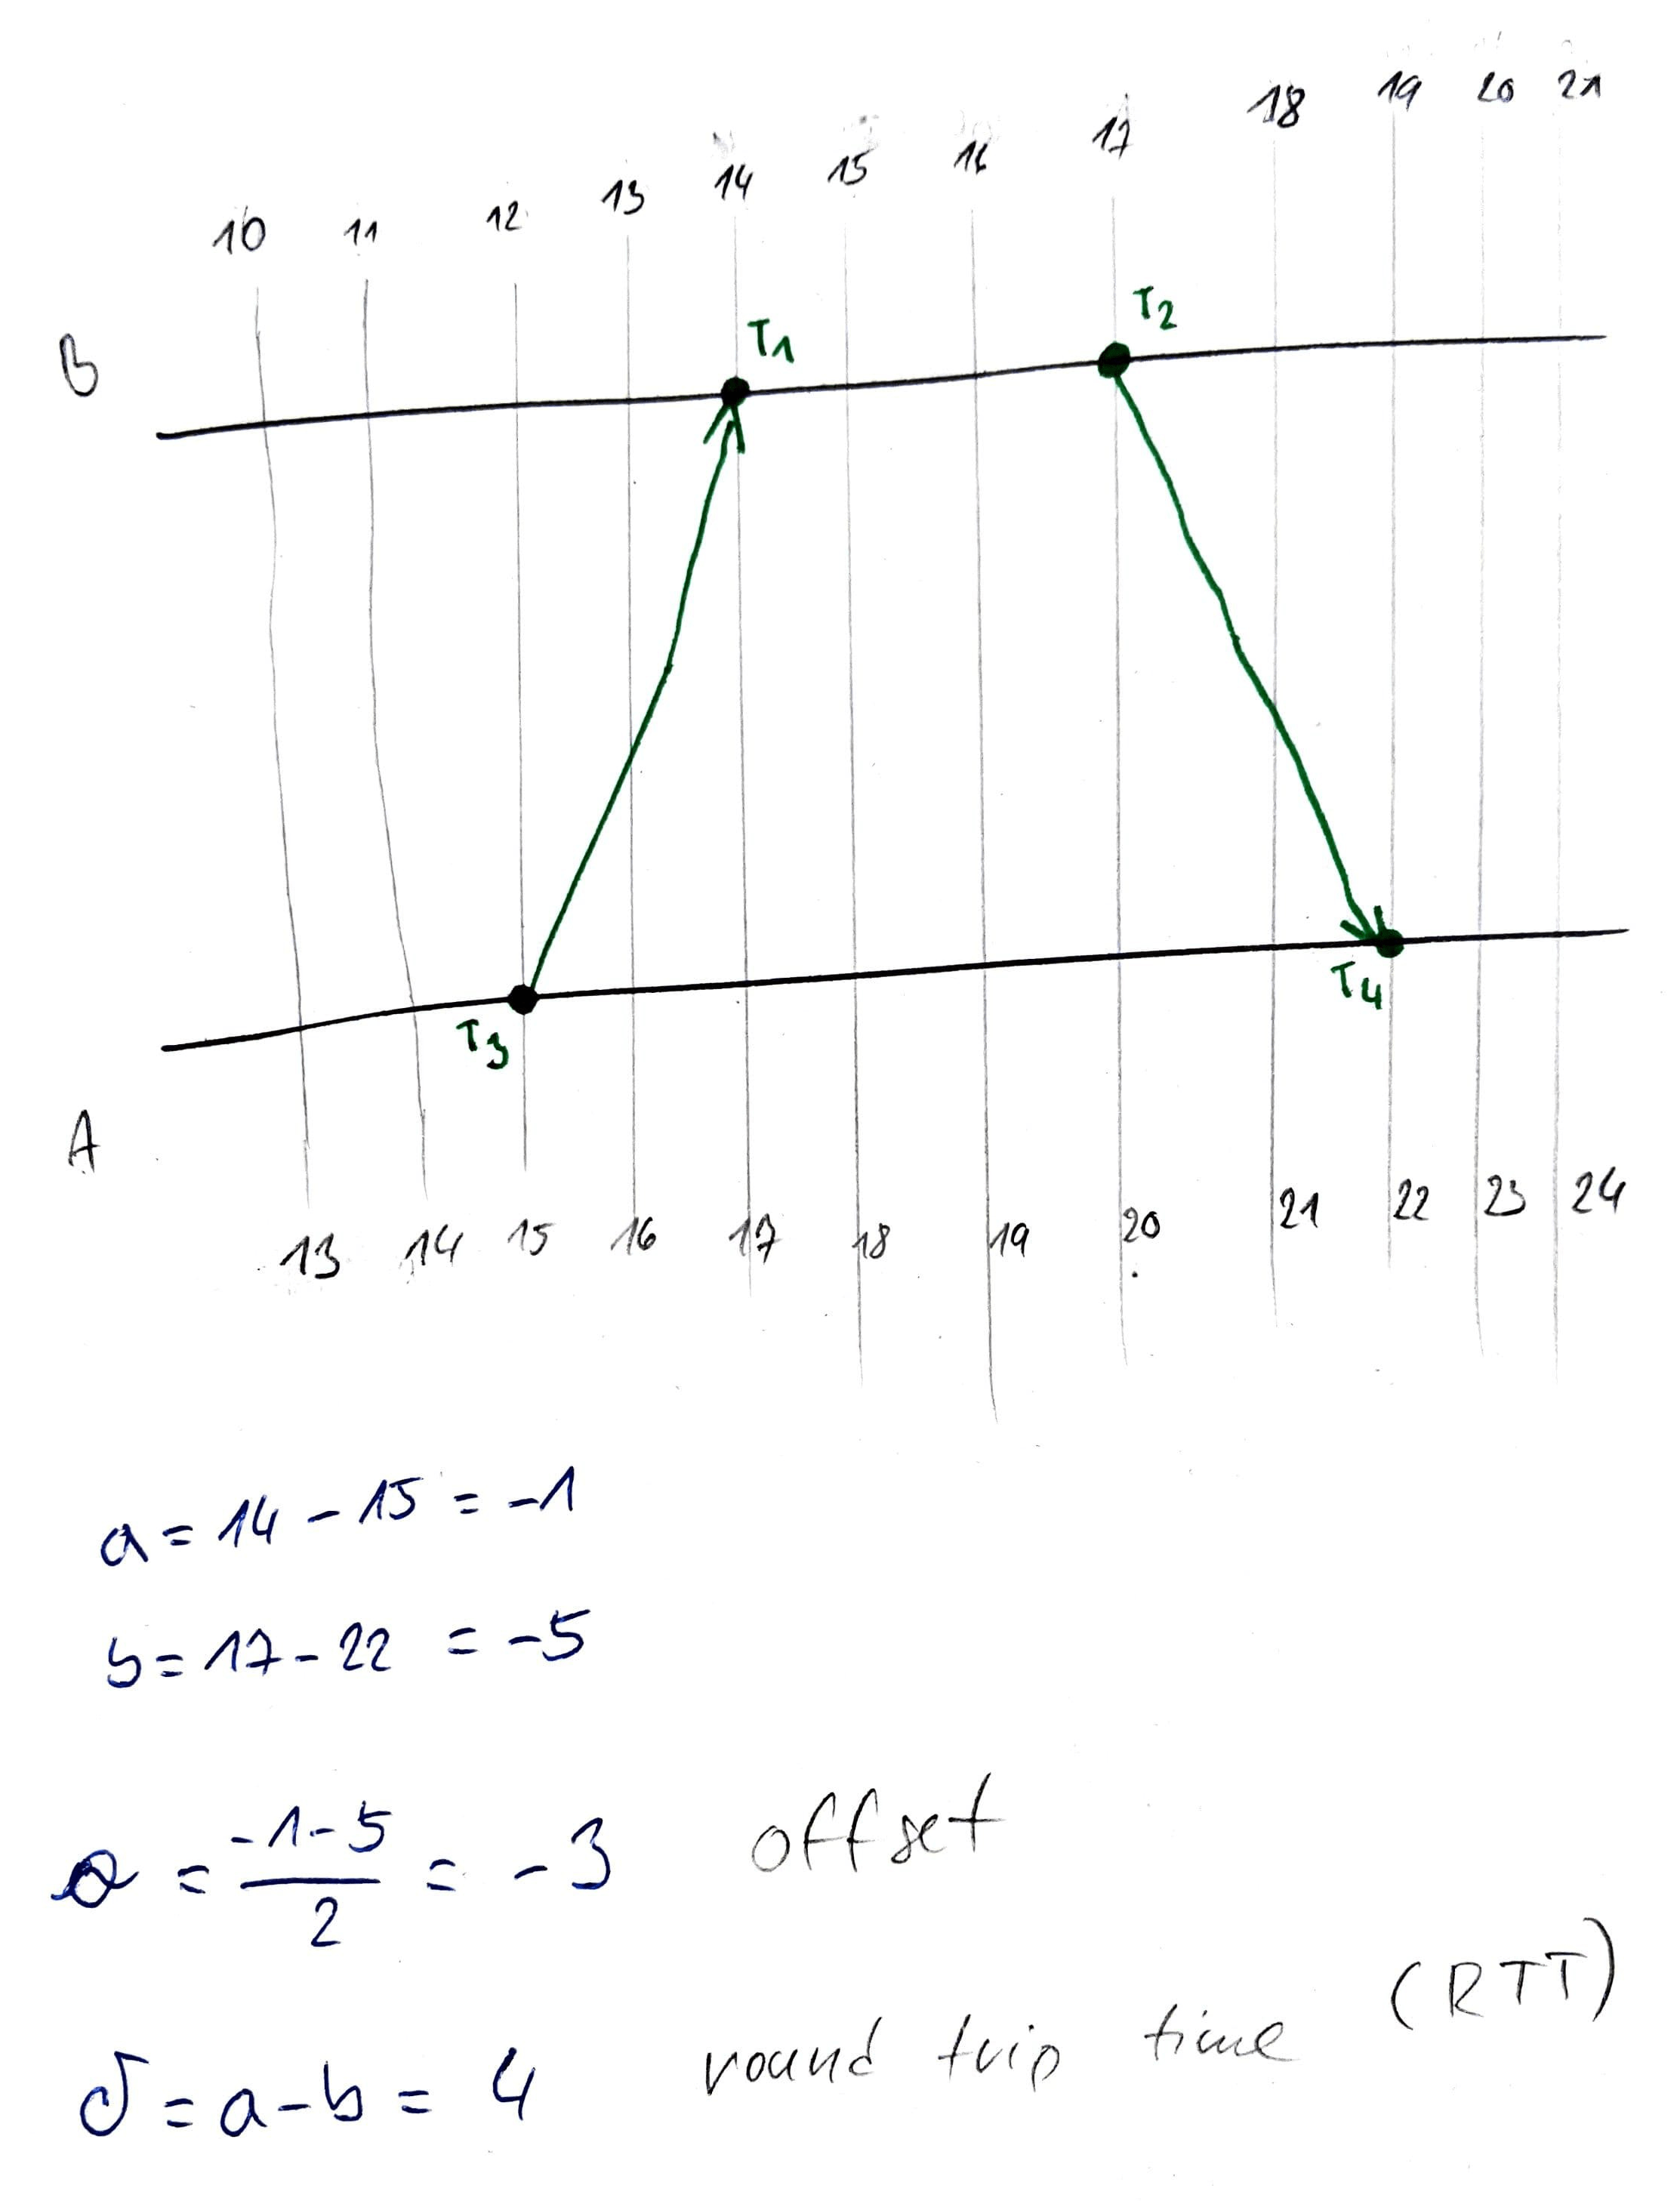
\includegraphics[width=1\linewidth]{ntp_priklad_2.png}
        \caption{Další příklad uzlů s fyzickým časem.}
    \end{figure}

\end{compactitem}

%%%%%%%%%%%%%%%%%%%%%%%%%%%%%%%%%%%%%%%%%%%%%%%%%%%%%%%%%%%%%%%%%%%%%%%%%%%%%%%%

\section{Synchronizace řízená koordinátorem}

\begin{compactitem}
    \item Chceme vybrat koordinátora (\textit{master}, hlavní uzel). \begin{compactitem}
        \item Koordinátora lze využít pro centralizovanou správu přístupu ke kritické sekci. Koordinátor monitoruje stav sdíleného zdroje a udržuje frontu pro přístup.
    \end{compactitem}

    \item Předpokládáme:
    \begin{compactitem}
        \item Každý proces má unikátní ID.
        \item Procesy neznají stav (běžící, neběžící) dalších procesů.
        \item Každý proces zná ID dalších procesů (záleží na topologii).
    \end{compactitem}
    \item Cíl:
    \begin{compactitem}
        \item Dosáhnutí shody mezi všemi procesy na procesu, který je koordinátor.
        \item Kritérium výběru koordinátora může být různé. Např. na základě proces ID (proces s~největším ID se stane koordinátorem).
    \end{compactitem}
\end{compactitem}

\subsection{Chang Roberts algoritmus}

\begin{compactitem}
    \item \textit{Toto je v podstatě Ring algoritmus z PDI, viz otázku~\ref{chapter_pdi_koordinator}. Ring algoritmus používá seznam a díky tomu ušetří jedno kolo zpráv, tj. vyšší prostorová složitost výměnou za lepší časovou.}

    \item Předpokládá kruhovou topologii.
    \item Hledá maximální hodnotu PID.
    \item Zprávy jsou posílány po směru hodinových ručiček.

    \item \textbf{Postup} \begin{compactenum}
        \item Uzel zahájí komunikaci, označí se za účastníka a pošle zprávu se svým ID následujícímu.
        \item Pokud uzel přeposílá zprávu, označí se za účastníka.
        \item Každý uzel po obdržení zprávy: \begin{compactenum}
            \item Pokud ID ve zprávě je větší než ID tohoto uzlu, je zpráva přeposlána dále tak jak je.
            \item Pokud je číslo ve zprávě menší než má uzel ID, potom: \begin{compactenum}
                \item Pokud již je účastník, zahodí zprávu.
                \item Pokud není účastník, nahradí hodnotu původní za svoje ID a přepošle zprávu dále.
            \end{compactenum}
            \item Pokud je číslo ve zprávě stejné jako má uzel ID, potom tento uzel volbu vyhrál. Potom zahájí druhou část algoritmu.
        \end{compactenum}
        \item Vítěz volby se odznačí jako účastník a pošle svoje číslo dále.
        \item Každý, kdo obdrží zprávu a je stále účastníkem, si číslo poznačí, odznačí se jako účastník a pošle zprávu dále.
        \item Pokud zprávu obdrží vítěz volby, zprávu zahodí.
    \end{compactenum}

    \item \textbf{Složitost} \begin{compactitem}
        \item V nejhorším případě se musí přeposlat $3(n-1)$ zpráv.
        \item Nejhorší případ -- uzel s maximálním indexem je první za iniciátorem hlasování.
    \end{compactitem}

    \begin{figure}[H]
        \centering
        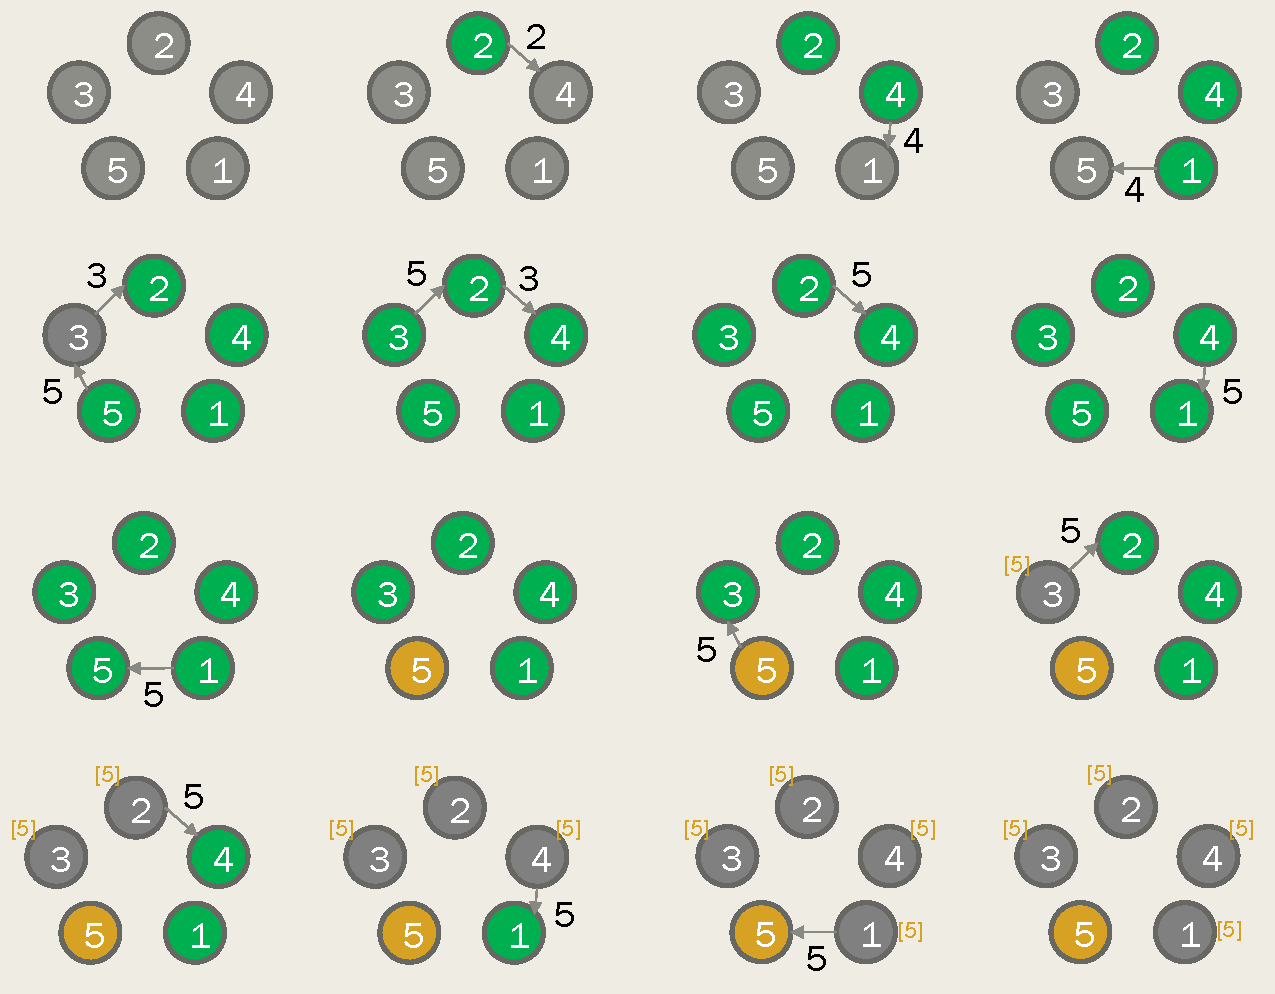
\includegraphics[width=1\linewidth]{chang_roberts.pdf}
        \caption{Příklad činnosti Chang-Roberts algoritmu.}
    \end{figure}
\end{compactitem}

%%%%%%%%%%%%%%%%%%%%%%%%%%%%%%%%%%%%%%%%%%%%%%%%%%%%%%%%%%%%%%%%%%%%%%%%%%%%%%%%

\section{Synchronizace logickým časem}

\begin{compactitem}
    \item Procesy hledají shodu navzájem na tom, který z nich získá kritickou sekci.

    \item Známe 2 mechanismy (třídy algoritmů) vzájemného vyloučení v distribuovaných systémech.

    \item Algoritmy založené na časových razítcích: \begin{compactitem}
        \item Lamportův algoritmus
        \item Algoritmus Ricart-Agrawala
        \item Meakawův algoritmus
    \end{compactitem}

    \item Algoritmy založené na tokenech: \begin{compactitem}
        \item Raymondův algoritmus
        \item Suzuki-Kasami vysílací algoritmus
    \end{compactitem}
\end{compactitem}

\subsection{Logické (Lamportovy) hodiny}

\begin{compactitem}
    \item Vytvoření tzv. logického času pomocí relace \textit{happened before}. \begin{compactitem}
        \item Relace $R_{HB}(e_1, e_2)$ značí: \begin{compactitem}
            \item událost $e_1$ předchází $e_2$ v rámci jednoho procesu;
            \item událost $e_1$ je $send(p_2, m)$ v rámci procesu $p_1$ a $recv(p_1, m)$ je událost $e_2$ v rámci procesu $p_2$.
        \end{compactitem}

        \item $R_{HB}$ je tranzitivní, nereflexivní relace částečného uspořádání.

        \item Abychom dosáhli úplného uspořádání je třeba dodat další informaci, zde lze použít ID procesů, pak procesy s nižším číslem \uv{mají přednost} a jejich události, pro které nemůžeme uspořádání původně určit, předcházejí událostem procesů s vyšším číslem.

        \item Nerozlišujeme zvýšení logického času na základě toho, jestli k němu došlo vnitřní událostí, nebo na základě komunikace.
    \end{compactitem}

    \item \textbf{Definice} \begin{compactitem}
        \item Logické hodiny $C$ jsou funkce $C : E \rightarrow T$, kde \begin{compactitem}
            \item $E$ je konečná množina událostí;
            \item $T$ je časová doména (např. $\mathbb{N}$) nad kterou je definována relace částečného uspořádání ($<$).
        \end{compactitem}

        \item Každý proces $P_i$ má své logické hodiny $C_i$.
        \item Logické hodiny před každou událostí $e$ inkrementují čítač.
        \item $C(e)$ vrací pro každou událost odpovídající logický čas.

        \item Pro konzistentní hodiny požadujeme:
        $$ \forall (e_1, e_2) \in E : R_{HB}(e_1, e_2) \Rightarrow C(e_1) < C(e_2) $$
    \end{compactitem}

    \item \textbf{Implementace} \begin{compactitem}
        \item Spolu se zprávou se posílá i časové razítko dle logického času vysílacího procesu.

        \item Při přijetí zprávy $recv(p, m, t_p)$ si příjemce aktualizuje svůj logický čas:
        $$ C_i = max(C_{i} + 1, t_{p} + 1) $$
    \end{compactitem}

    \begin{figure}[H]
        \centering
        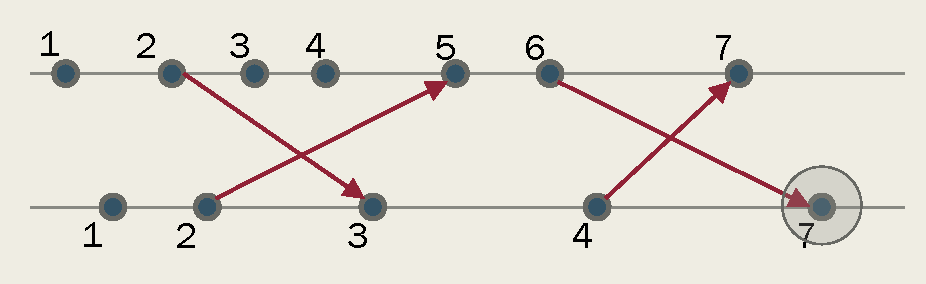
\includegraphics[width=1\linewidth]{logicke_hoginy.pdf}
        \caption{Příklad komunikace dvou procesů a logických hodin.}
    \end{figure}
\end{compactitem}

\subsection{Lamportův algoritmus}

\begin{compactitem}
    \item Založeno na FIFO doručování zpráv.
    \item Udržuje lokální prioritní frontu zpráv ve které priority jsou úplně uspořádány podle předávaných časových razítek.

    \item Složitost: Lamportův algoritmus vyžaduje $3(n-1)$ zpráv: \begin{compactitem}
        \item $(n-1)$ požadavků;
        \item $(n-1)$ odpovědí;
        \item $(n-1)$ uvolnění.
    \end{compactitem}

    \begin{figure}[H]
        \centering
        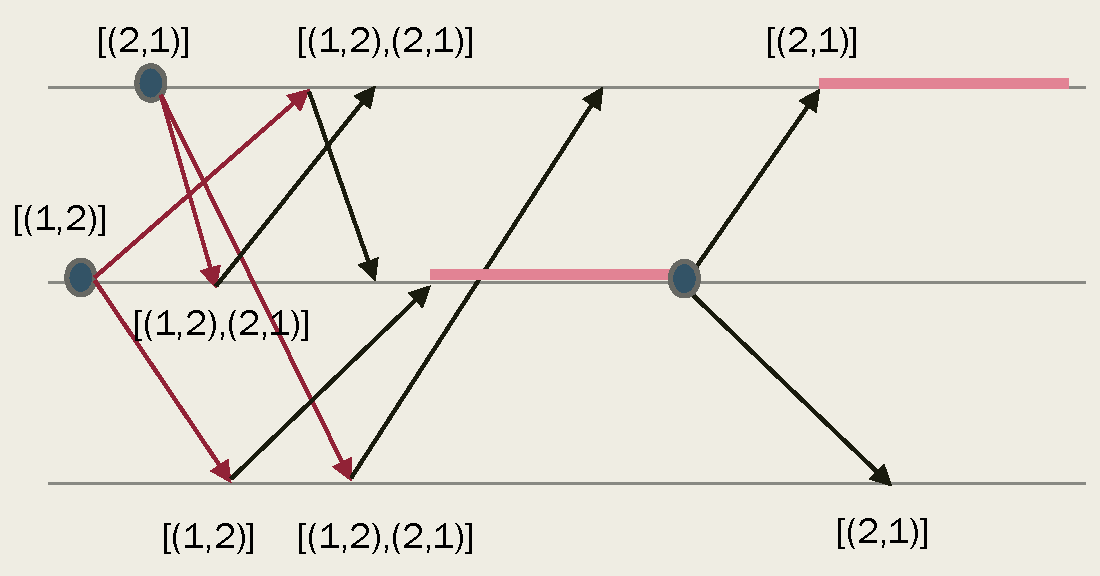
\includegraphics[width=1\linewidth]{lamportuv_algoritmus.pdf}
        \caption{Příklad Lamportova algoritmu. Časová razítka obsahují navíc i ID procesu a díky tomu jsou úplně uspořádána. Červenou čarou je zvýrazněn přístup do kritické sekce.}
    \end{figure}
\end{compactitem}

\subsection{Raymondův algoritmus}

\begin{compactitem}
    \item Jeden token reprezentuje v systému jednu kritickou sekci.
    \item Proces může vstoupit do kritické sekce, pokud obdrží token.
    \item Důkaz o vzájemném vyloučení procesu je triviální (token může držet jen jeden proces a ten jej předává, pokud není v kritické sekci).
    \item Předpokládá stromovou uspořádanou strukturu.

    % \item Vlastnosti: \begin{compactitem}
    %     \item nezpůsobuje vyhladovění;
    %     \item nezpůsobuje uváznutí;
    %     \item \textit{fault tolerance}.
    % \end{compactitem}

    \item Analýza: \begin{compactitem}
        \item Počet zaslaných zpráv -- třída složitosti $\mathcal{O}(\log{N})$.
        \item Průměrné synchronizační zpoždění je $\log{\frac{N}{2}}$.
        \item Přenosnost se snižuje při zahlcení sítě zprávami.
        \item Může použít greedy strategii -- možnost hladovění.
    \end{compactitem}

    \begin{figure}[H]
        \centering
        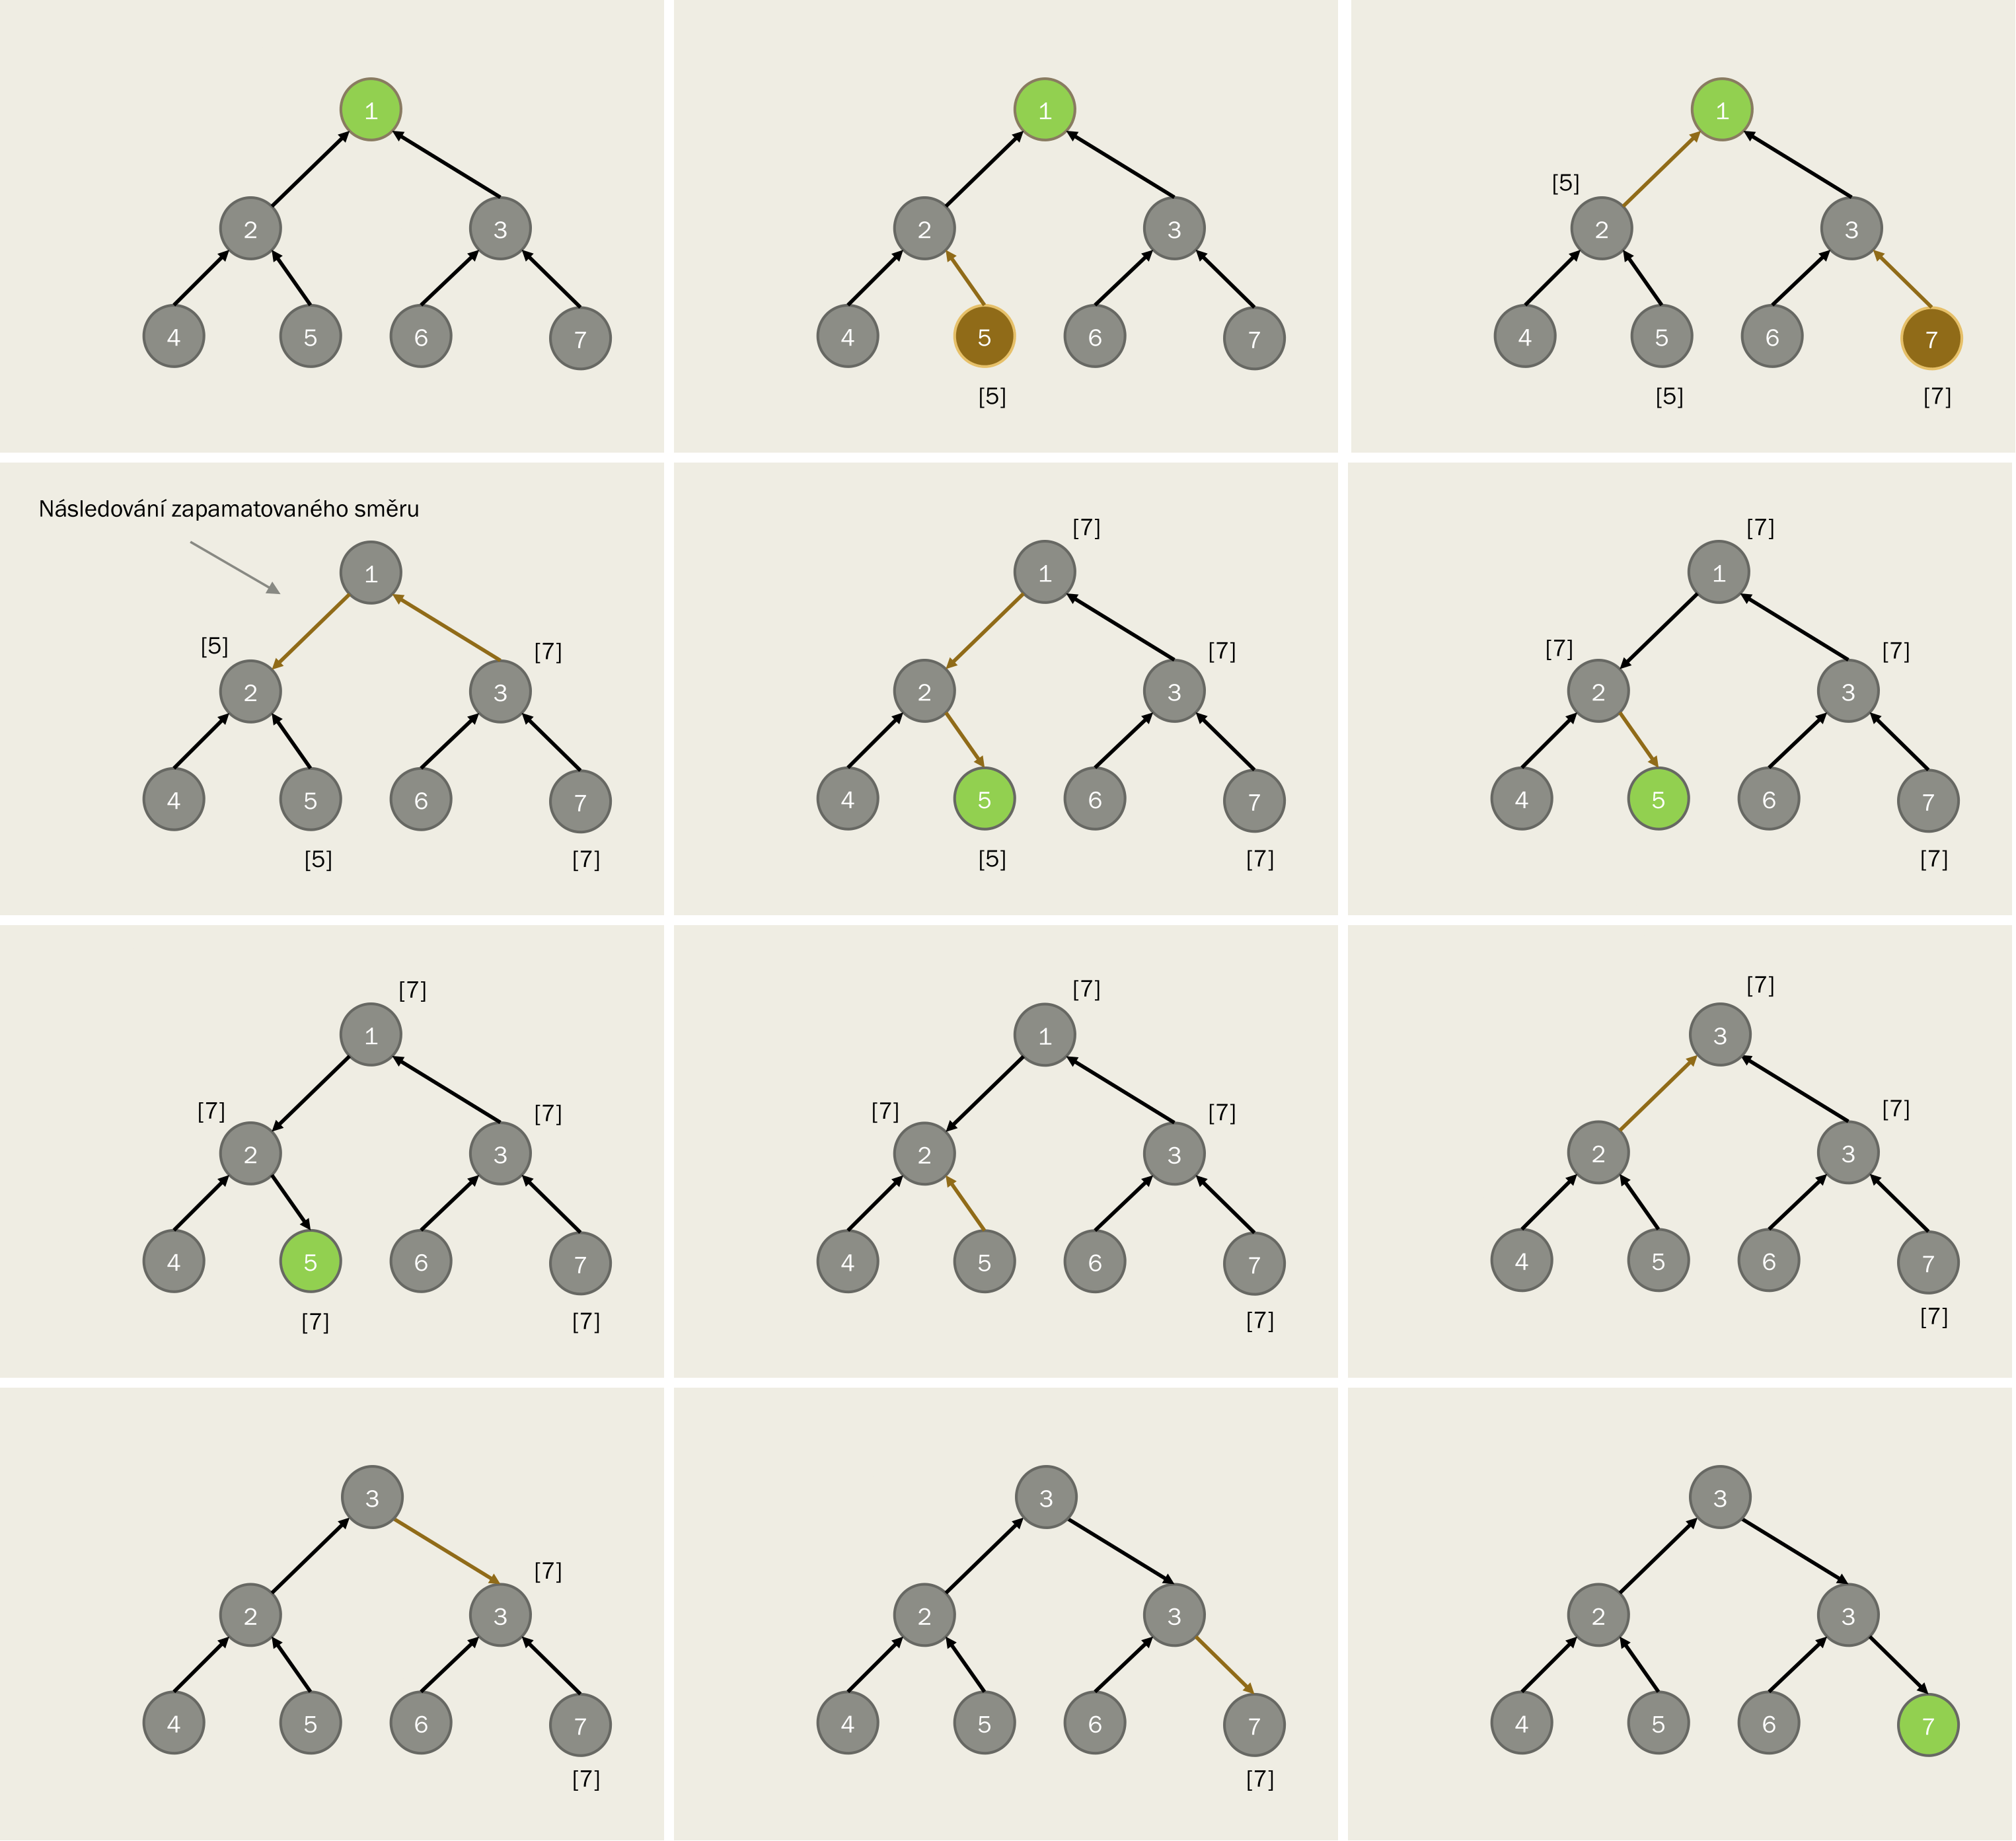
\includegraphics[width=1\linewidth]{raymonduv_algoritmus.png}
        \caption{Příklad Raymondova algoritmu. Zeleně je označen proces s přístupem do kritické sekce. Hnědě proces, který o kritickou sekci žádá.}
    \end{figure}
\end{compactitem}

%%%%%%%%%%%%%%%%%%%%%%%%%%%%%%%%%%%%%%%%%%%%%%%%%%%%%%%%%%%%%%%%%%%%%%%%%%%%%%%%

\section{Distribuovaný broadcast}

% todo: priklad, kauzalni, ktery neni uplny a uplny, ktery neni kauzalni

\begin{compactitem}
    \item Distribuovaný broadcast $\sim$ všesměrové vysílání.

    \item Předpoklady pro broadcast: \begin{compactitem}
        \item Známé největší možné zpoždění při doručování zprávy.
        \item Lokální hodiny pro každý z procesů.
        \item Známý nejvyšší časový limit pro vykonání interní akce.
        \item Topologie sítě je obecná.
    \end{compactitem}

    \item Vlastnosti \begin{compactitem}
        \item \textbf{Platnost} (\textit{validity}) -- Pokud zpráva byla odeslána korektním procesem, tak v konečném čase ji každý další proces obdrží.

        \item \textbf{Shoda} (\textit{agreement}) -- Pokud zpráva byla obdržena korektním procesem, pak v konečném čase ji obdrží všechny procesy.

        \item \textbf{Integrita} (\textit{integrity, no duplication}) -- Žádná zpráva není doručena více než jednou.

        \item \textbf{Opravdovost} (\textit{no creation}) -- Pokud proces obdržel zprávu $m$ od procesu $p$, pak tento proces zprávu opravdu odeslal.
    \end{compactitem}

    \item Vlastnosti z hlediska pořadí doručování \begin{compactitem}
        \item \textbf{FIFO uspořádání} -- Pokud proces broadcastne zprávu $m$ a poté zprávu $n$, pak každý proces obdrží nejprve $m$ a poté až $n$ (FIFO uspořádání od jednoho procesu).

        \item \textbf{Kauzální uspořádání} -- Pokud broadcast zprávy $m$ předchází broadcastu zprávy $n$, pak každý proces obdrží nejprve $m$ a poté až $n$ (FIFO uspořádání od všech procesů).

        \item \textbf{Úplné uspořádání} -- Pokud procesy $p$ a $q$ oba obdrží zprávu $m$ a $n$, pak $p$ obdrží $m$ před $n$ pokud $q$ obdrží zprávu $m$ před $n$ (přijímají z pohledu příjemců ve stejném pořadí všechny procesy).
    \end{compactitem}

    \item Klasifikace \begin{compactitem}
        \item Best effort broadcast -- platnost (shoda nikoliv, protože nekorektní proces odešle pouze podmnožině korektních).
        \item Spolehlivý (reliable) broadcast -- platnost, shoda a integrita.
        \item FIFO broadcast -- spolehlivý a FIFO uspořádání.
        \item Kauzální broadcast -- spolehlivý a kauzální uspořádání.
        \item Atomický broadcast -- spolehlivý, FIFO uspořádání a kauzální uspořádání.
        \item Kauzálně atomický broadcast -- spolehlivý, kauzální uspořádání a úplné uspořádání.
    \end{compactitem}

    \begin{figure}[H]
        \centering
        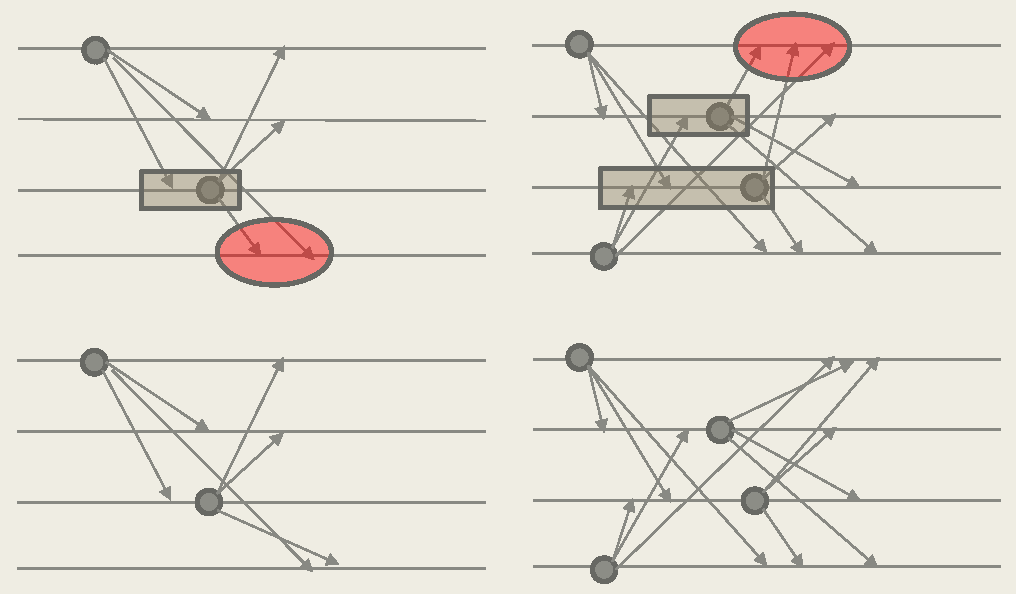
\includegraphics[width=1\linewidth]{broadcast.pdf}
        \caption{Příklad broadcastu.}
    \end{figure}
\end{compactitem}
